% Preamble
% Compile with XeLateX

\documentclass[11 pt,oneside,a4paper,titlepage]{article}
\usepackage{preamble}
\graphicspath{{PIC/}}
%%%%%%%%%%%%%%%%%%%%%%%%%%%%%%%%%%%%%%%%%%%%%%%%%%%%%%%%%%%%%%%%%%%%%%%%%%%%%%%%%%%%%%
\begin{document}

\sidebar{sideBarColor!25}
\simpleheader{titleBackColor}{Grover}{Aruquipa}{Mechatronics | Engineer}{white}

% Start Minipages
\vspace*{3.49cm}% start 8 cm from the top of the page}
    \adjustbox{valign=t}{\begin{minipage}{7.3cm} % large 7.4 cm from the top
    \vspace*{1.2cm} % text starts 1cm under the top of the minipage
            
        % Picture
        \begin{center}
        \begin{tikzpicture}
            \node[
            circle,
            minimum size=\cvPictureWidth,
            path picture={
            \node at (path picture bounding box.center){
             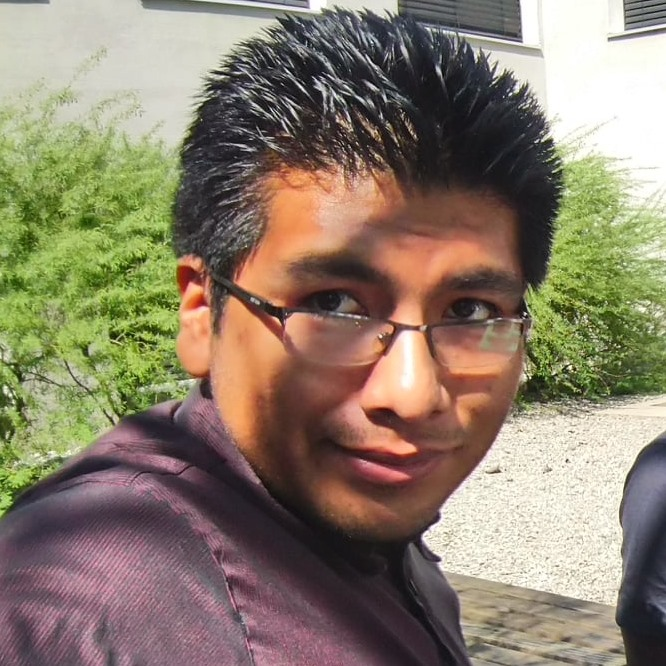
\includegraphics[width=\cvPictureWidth]{Picture.jpg}
             };
             }]
            {};
        \end{tikzpicture}
        \end{center}

        %%%%%%%%%%%%%%%%%%%%%%%%%%%%%%%%%%%%%%%%%%%%%%%%%%%%
        % Profile section
        \ruleline{\textbf{About me}}
        %\lipsum[150] %
        I am mechatronics engineer passionated for the parallel robots
        %%%%%%%%%%%%%%%%%%%%%%%%%%%%%%%%%%%%%%%%%%%%%%%%%%%
        % Contact Section
        \ruleline{\textbf{Contact}}
        \begin{tikzpicture}[every node/.style={inner sep=0pt, outer sep=0pt}]
        \matrix [
        column 1/.style={anchor=center,contactIcon},
        column 2/.style={anchor=west,align=left,contactIcon},
        column sep=5pt,
        row sep=5pt] (contact) {
        \node{\faMale};
         & \node{Born on 09/09/1995, Age 27};\\
        \node{\faEnvelope}; 
         & \node{\href{mailto:jacksparrow@yahoo.it}{grover.aruquipa.9@gmail.com}};\\
         \node{\faEnvelopeO}; 
         & \node{\href{mailto:jacksparrow2@yahoo.it}{grover.aruquipa@femto-st.com}};\\
        \node{\faPhone}; 
         & \node{+33 629779225};\\ 
        \node{\faMapMarker}; 
        & \node{l'ephitaphe 9 \\ 25000 Besancon , France};\\
        \node{\faLinkedinSquare}; 
        & \node{\href{https://www.linkedin.com/in/grover-aruquipa-996917126}{GroverAruquipa}};\\
        \node{\aiResearchGateSquare}; 
        & \node{\href{https://www.researchgate.net/profile/Grover-Aruquipa}{Research Gate: Grover Aruquipa}};\\
        \node{\aiOrcid}; 
        & \node{\href{https://orcid.org/my-orcid?orcid=0000-0003-0243-3187}{ORCID: 0000-0003-0243-3187}};\\
        
        \node{\faGithub};
        & \node{\href{https://groveraruquipa.github.io/}{Github: Grover Aruquipa}};\\
        \node{\faGear};
        & \node{\href{https://grabcad.com/grover.aruquipa-2}{Grabcad: Grover Aruquipa}};\\
        \\
         };
        \end{tikzpicture} 
        
        %%%%%%%%%%%%%%%%%%%%%%%%%%%%%%%%%%%%%%%%%%%%%%%%%%%
        \ruleline{\textbf{Languages}}
        \begin{tikzpicture}[every node/.style={inner sep=0pt, outer sep=0pt}]
        \matrix [
        column 1/.style={anchor=center,contactIcon},
        column 2/.style={anchor=west,align=left,contactIcon},
        column sep=5pt,
        row sep=5pt] (contact) {
        \node{\flag{Spain.png}};
        & \node{Spanish - Native Language};\\
        \node{\flag{England.png}};
        & \node{English - Professional Knowledge};\\
        \node{\flag{France.png}};
        & \node{French - Basic Knowledge};\\
        \node{\flag{german.png}};
        & \node{German - Basic Notions};
        \\
        };
        \end{tikzpicture} 
        
        %%%%%%%%%%%%%%%%%%%%%%%%%%%%%%%%%%%%%%%%%%%%%%%%%%%%%
        % QR Code
        \begin{center}
            
\includegraphics[width=3.5cm]{QR_Info.png}
        \end{center}
        
    \end{minipage}} %
    \hfill 
%%%%%%%%%%%%%%%%%%%%%%%%%%%%%%%%%%%%%%%%%%%%%%%%%%%%%%%%%
%%%%% MAIN SECTION %%%%%%%%%%%%%%%%%%%%
    \adjustbox{valign=t}{\begin{minipage}{11.3cm}
        \vspace*{1cm}
        \section*{{\faGraduationCap} EDUCATION}

        \MySection{2022-Ongoing}{Books.png}{Master 2 Degree}{University Franche Comte}{Besancon, France}{Faculty}{Avrage. \\\textbf{ X }}
       \vspace*{0.22cm}
       \MySection{2021-2022}{Books.png}{Master 1 Degree}{University Franche Comte}{Besancon, France}{Faculty}{ \\\textbf{Avrage: x0}}

         \vspace*{0.22cm}
            
        \MySection{2019-2022}{Books.png}{Engineer Specialization}{Robotics and Automation}{Bolivian Catholic University}{Buccaneer}{Bachelor Thesis. \\\textbf{Degree: 90/100}}
            
        \vspace*{0.22cm}
            
        \MySection{2014-2019}{Books.png}{Bachelor Degree}{Mechatronics Engineer}{Bolivian Catholic University}{Buccaneer}{Bachelor Thesis. \\\textbf{Degree: 90/100}}


                
        %%%%%%%%%%%%%%%%%%%%%%%%%%%%%%%%%%%%%%%%%%%%%%%%%%%
        % Work Experience
        \section*{{\faSuitcase} WORK EXPERIENCE}
            
        \MySectionNoPic{2022-Today}{Research inter}{Besancon, France}{Femto-st}{Researching in parallel robots }  
            
        \vspace*{0.22cm}
            
        \MySectionNoPic{2021}{Computer Vision Engineer}{La Paz, Bolivia}{Debveloping Computer vision solutions.}  
        
        \vspace*{0.22cm}
            
        \MySectionNoPic{2021}{Data Scientist}{\textit{Virtual}}{KTH}{Debveloping analysis of dataset for environment impact.}

        \vspace*{0.22cm}

        \MySectionNoPic{2020}{Graduated intern}{Zurich, Switzerland}{HTACHI-ABB}{Analysis of complex Datasets.}

        %%%%%%%%%%%%%%%%%%%%%%%%%%%%%%%%%%%%%%%%%%%%%%%%%%%
        % Publications
        \section*{{\aiOBP} PUBLICATIONS}
            
        \publication{Journal Article}{1729}{An IoT architecture based on the control of Bio Inspired manufacturing system for the detection of anomalies with vibration sensors}{Grover Aruquipa, Fabio Diaz}{ScienceDirect}{https://doi.org/10.1016/j.procs.2022.01.242}
            
        \vspace*{0.22cm}
             
        \publication{Conference Article}{1725}{ Analysis of Algorithmic Trading with Q-Learning in the Forex Market}{Grover Aruquipa, Gabriel Rojas}{IEEE-2021 International Conference on Emerging Smart Computing and Informatics}{10.1109/ICMIMT52186.2021.9476134}
            
        \vspace*{0.22cm}
            
        \publication{Conference Article}{1724}{Design and Implementation of a Delta Robot Based on FPGA for the Automation of the Collection of Solid Products}{Grover Aruquipa, Gabriel Rojas}{IEEE - International Conference on Industrial Engineering, Applications and Manufacturing  }{10.1109/ICIEAM51226.2021.9446417}
            
        \vspace*{0.22cm}
        
        \publication{Conference Article}{1724}{How I lost my ship and how to get it back}{Jack Sparrow}{Conference in Tortuga}{10.5220/doidoidoi}
            
        \vspace*{0.22cm}
            
    \end{minipage}} %

%%%%%%%%%%%%%%%%%%%%%%%%%%%%%%%%%%%%%%%%%%%%%%%%%%%%%%%%%%%%
% Second Page
\newpage

\sidebar{sideBarColor!25}
\newpageheader{titleBackColor}{Grover}{Aruquipa}{Mechatronics \faLightbulbO \hspace{1mm} Engineer}{white}

% %%%%%%%%%%%%%%%%%%%%%%%%%%%%%%%%%% SIDEBAR %%%%%%%%%%%%%%%%%%%
\adjustbox{valign=t}{%
\begin{minipage}{7.3cm} 
\vspace*{0.4cm} % text starts 0.4cm under the top the header
        
    %%%%%%%%%%%%%%%%%%%%%%%%%%%%%%%%%%%%%%%%%%%%%%%%%%%%
    % Skill and Strengths 
    \ruleline{\textbf{Soft Skills and Strengths}}
    \vspace*{-0.5cm}
    \begin{center}
        \cvtag{Curiosity}\cvtag{Flexibility}\cvtag{Self Confidence}\cvtag{Ability to Plan and Organize} \cvtag{Autonomy}\cvtag{Adaptability} \cvtag{Eye for Details}\cvtag{Problem Solving}\cvtag{Team Working}\cvtag{Love Learning New Things}\cvtag{Leadership}\cvtag{Good Communication}\cvtag{Managing Information}\cvtag{Diplomacy}\cvtag{Good Listener}\cvtag{Patience}
    \end{center}

    %%%%%%%%%%%%%%%%%%%%%%%%%%%%%%%%%%%%%%%%%%%%%%%%%%%%
    % Professional Skills 
    \ruleline{\textbf{Professional Skills}}
    \begin{center}
        \cvtag{Bio-Insperd Algorithms}\cvtag{Screw Theory}\cvtag{Control Systems}\cvtag{Parallel Robots}\cvtag{Syntesis of Mechanism}
    \end{center}

    %%%%%%%%%%%%%%%%%%%%%%%%%%%%%%%%%%%%%%%%%%%%%%%%%%%
    % Other Interests
    \ruleline{\textbf{Other Interests}}
    \small
    \begin{multicols}{2}
        \begin{itemize} 
            \item  Research \flag{Books.png}
            \item  Programming \flag{Piano.png}
            \item  Chess \flag{Chess.png}
            \item  Gym \flag{Gym.png}
            \item  3D Printers \flag{Travels.png}
            \item  Trading \flag{movie2.png}
            \item  Salsa Dance \flag{Books.png}
    \end{itemize}
    \end{multicols}

     %%%%%%%%%%%%%%%%%%%%%%%%%%%%%%%%%%%%%%%%%%%%%%%%%%%%%
        % QR Code
        \ruleline{\textbf{Download My CV}}
        \scriptsize
        \centering
        Download my CV via the QR below \aiOverleaf.
        \begin{center}
            \quad
            \qrcode[height=2cm]{
                https://www.dropbox.com/sh/k5pheguf9jrur8x/AADpyjYJi7V5bhPyJeP3H74ea?dl=0} \\
            \vspace*{0.5cm}
        \end{center}

\end{minipage}
}%
\hfill
%%%%%%%%%%%%%%%%%%%%%%%%%%%%%%%%%%% MAIN %%%%%%%%%%%%%%%%%%%%%%%%%
\adjustbox{valign=t}{%
\begin{minipage}{11.3cm}
    \vspace*{0.4cm}
    %%%%%%%%%%%%%%%%%%%%%%%%%%%%%%%%%%%%%%%%%%%%%%%%%%%
    % Peer Reviews
    \section*{{\faBook} ACADEMIC PEER REVIEWS}
    \footnotesize I did academic peer review for the following journals: 
    \begin{itemize}
        \footnotesize
         \item{\textbf{Editor SETRE}, September 2021;}
         \item{\textbf{ISM 2021},ISM(International Conference on Industry 4.0 and Smart Manufacturing (ISM)), November 2021;}
     \end{itemize}
        
    %%%%%%%%%%%%%%%%%%%%%%%%%%%%%%%%%%%%%%%%%%%%%%%%%%%
    % Information Technology Skills
    \section*{{\faDesktop} INFORMATION TECHNOLOGY SKILLS}
    
    \ITCcompetence{Data Analysis}{
    \textbf{MATLAB}: \textit{Higly Specialized}\\
    \textbf{R-studio}: \textit{Higly Specialized}\\
    \textbf{Wolfram alpha}: \textit{Intermediate}\\
    
    }
    
    \vspace*{0.22cm}

    \ITCcompetence{Modeling and Simulation}{
    \textbf{Simulink} : \textit{Higly Specialized}  \\
    \textbf{Solidworks} : \textit{Higly Specialized}  \\
    \textbf{PTC-CREO} : \textit{Intermediate}  \\
    \textbf{Ansys}: \textit{Intermediate}\\
    \textbf{Labview}: \textit{Advanced}
    }
    
    \vspace*{0.22cm}

    \ITCcompetence{Frameworks}{
    \textbf{OpenCV} : \textit{Advanced}  \\
    \textbf{Tensorflow, Pytorch} : \textit{Advanced}  \\
    \textbf{Dash, Flashk, Django} : \textit{Advanced}  \\
    \textbf{ROS and ROS2} : \textit{Intermediante}  \\
    
    }

    \vspace*{0.22cm}

    \ITCcompetence{Office Automation}{
    \textbf{MS Office (Excel, Word, PowerPoint)}: \textit{Higly Specialized}\\
    \textbf{\LaTeX}: \textit{Advanced}\\
    }
    
    %%%%%%%%%%%%%%%%%%%%%%%%%%%%%%%%%%%%%%%%%%%%%%%%%%%
    % Programming Languages
    \section*{{\faCode} PROGRAMMING LANGUAGES}
    \vspace*{-0.5cm}
    \begin{multicols}{2}    
    \begin{itemize}
    \footnotesize
        \item \textbf{Matlab}: Highly Specialised
        \item \textbf{Python}: Advanced
        \item \textbf{SQL}: Intermediate
        \item \textbf{C/C++}: Advanced
        \item \textbf{Java}: Basic
        \item[\vspace{\fill}]
    \end{itemize}
    \end{multicols}
    
    %%%%%%%%%%%%%%%%%%%%%%%%%%%%%%%%%%%%%%%%%%%%%%%%%%%
    % Certificates
    \section*{{\faCertificate} CERTIFICATES}
    %%%%%%%%%%%%%%%%%%%%%%%%%%%%%%%%%%%%%%%%%%%%%%%%%%%%%%%%%
    \adjustbox{valign=t}{\begin{minipage}{2cm}
    \begin{center}
        
\includegraphics[width=1.2cm]{IBM.png}
    \end{center}
    \end{minipage}}
    \hfill \vline \hfill
    \adjustbox{valign=t}{\begin{minipage}{9cm}
        \begin{itemize}
            \scriptsize 
            \item IBM AI Engineering (\textit{Coursera, 2022})
        \end{itemize}
    \end{minipage}}

    \vspace*{0.6cm}
    
    \adjustbox{valign=t}{\begin{minipage}{2cm}
    \begin{center}
        
\includegraphics[width=1.2cm]{PIC/open-ai.jpg}
    \end{center}
    \end{minipage}}
    \hfill \vline \hfill
    \adjustbox{valign=t}{\begin{minipage}{9cm}
        \begin{itemize}
            \scriptsize 
            \item Generative Adversal Networks (\textit{Coursera, 2022})- Specialization
            \item Deep Learning (\textit{Coursera, 2020})-Specialization
            \item DeepLearning.AI TensorFlow Developer (\textit{Coursera, 2020})- Specialization
            
        \end{itemize}
    \end{minipage}}


    
    \vspace*{0.2cm}
    
    \adjustbox{valign=t}{\begin{minipage}{2cm}
    \begin{center}
        
\includegraphics[width=1.2cm]{PIC/google.png}
    \end{center}
    \end{minipage}}
    \hfill \vline \hfill
    \adjustbox{valign=t}{\begin{minipage}{9cm}
        \begin{itemize}
            \scriptsize 
            \item End-to-End Machine Learning with TensorFlow on Google Cloud (\textit{Coursera, 2020})- Course
            \item Machine Learning for Trading (\textit{Coursera, 2020})-Specialization
            
        \end{itemize}
    \end{minipage}}
    
    \vspace*{0.2cm}
    
    \adjustbox{valign=t}{\begin{minipage}{2cm}
    \begin{center}
        
\includegraphics[width=1.2cm]{PIC/edx.png}
    \end{center}
    \end{minipage}}
    \hfill \vline \hfill
    \adjustbox{valign=t}{\begin{minipage}{9cm}
        \begin{itemize}
            \scriptsize 
            \item A Hands-on Introduction to Engineering Simulations (\textit{Cornell University, 2020})
        \end{itemize}
    \end{minipage}}
    
    \vspace*{0.2cm}
    
    \adjustbox{valign=t}{\begin{minipage}{2cm}
    \begin{center}
        
\includegraphics[width=2.2cm]{PIC/coursera.jpg}
    \end{center}
    \end{minipage}}
    \hfill \vline \hfill
    \adjustbox{valign=t}{\begin{minipage}{9cm}
        \begin{itemize}
            \scriptsize 
            \item Reinforcement Learning Specialization (\textit{University of Alberta, 2020})
            \item Mathematics for Machine Learning Specialization (\textit{Imperial College London, 2020})
            \item Developing Industrial Internet of Things Specialization (\textit{University of Colorado Boulder, 2020})
            \item Digital Manufacturing \& Design Technology Specialization (\textit{University at Bufal, 2020})
            \item Digital Marketing Specialization (\textit{University of Illinois, 2020})
        \end{itemize}
    \end{minipage}}
    
    \vspace*{0.2cm}
    
\end{minipage}}


\end{document}
